% !TeX spellcheck = en_US

\chapter{Practical Results}\label{chp:practical_results}

\section{QGIS Plugin}
A QGIS plugin has been created, which allows to process the currently displayed imagery in a corresponding backend server. \autoref{fig:plugin:changes} shows an image of the imagery layer overlayed with the changes generated by the backend. The red dots on the upper left indicate deleted objects, or in other words, buildings that were not predicted in the image but were existent at the same location in the cadastral survey data. However, it is obvious, that in this case the neural network is wrong, as the actual buildings can be seen clearly. Additionally, in the lower middle the blue area can be seen, which indicates a change in the survey data.

A prediction is classified as change, as soon as it fully covers at least one existing object in the survey data. \autoref{fig:plugin:changes_cadastral_layer} shows the same changes on the cadastral data layer and \autoref{fig:plugin:predictions} shows the predictions as returned by the neural network.

\begin{figure}[H]
    \centering
	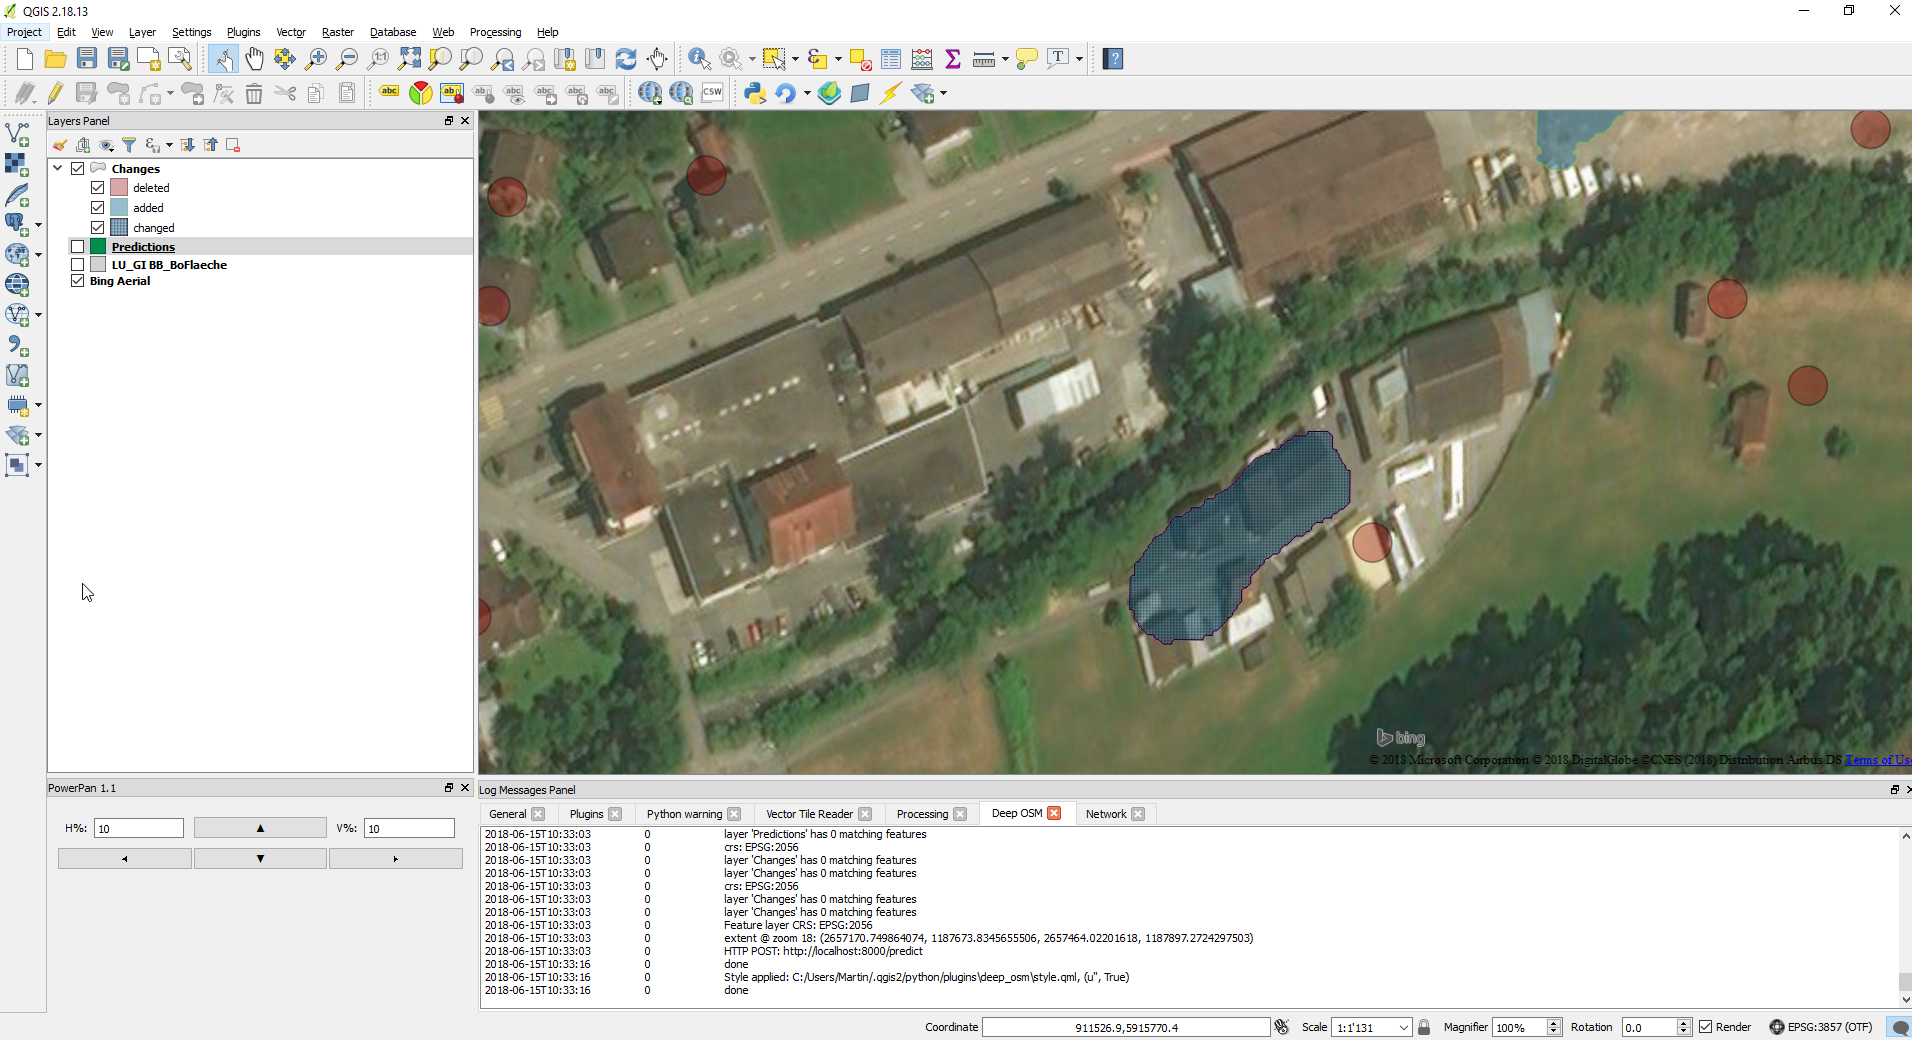
\includegraphics[width=1\linewidth]{chapters/practical_results/images/qgis_changes_aerial.png}
	\caption{Changes in QGIS}
	\label{fig:plugin:changes}
\end{figure}

\begin{figure}[H]
    \centering
	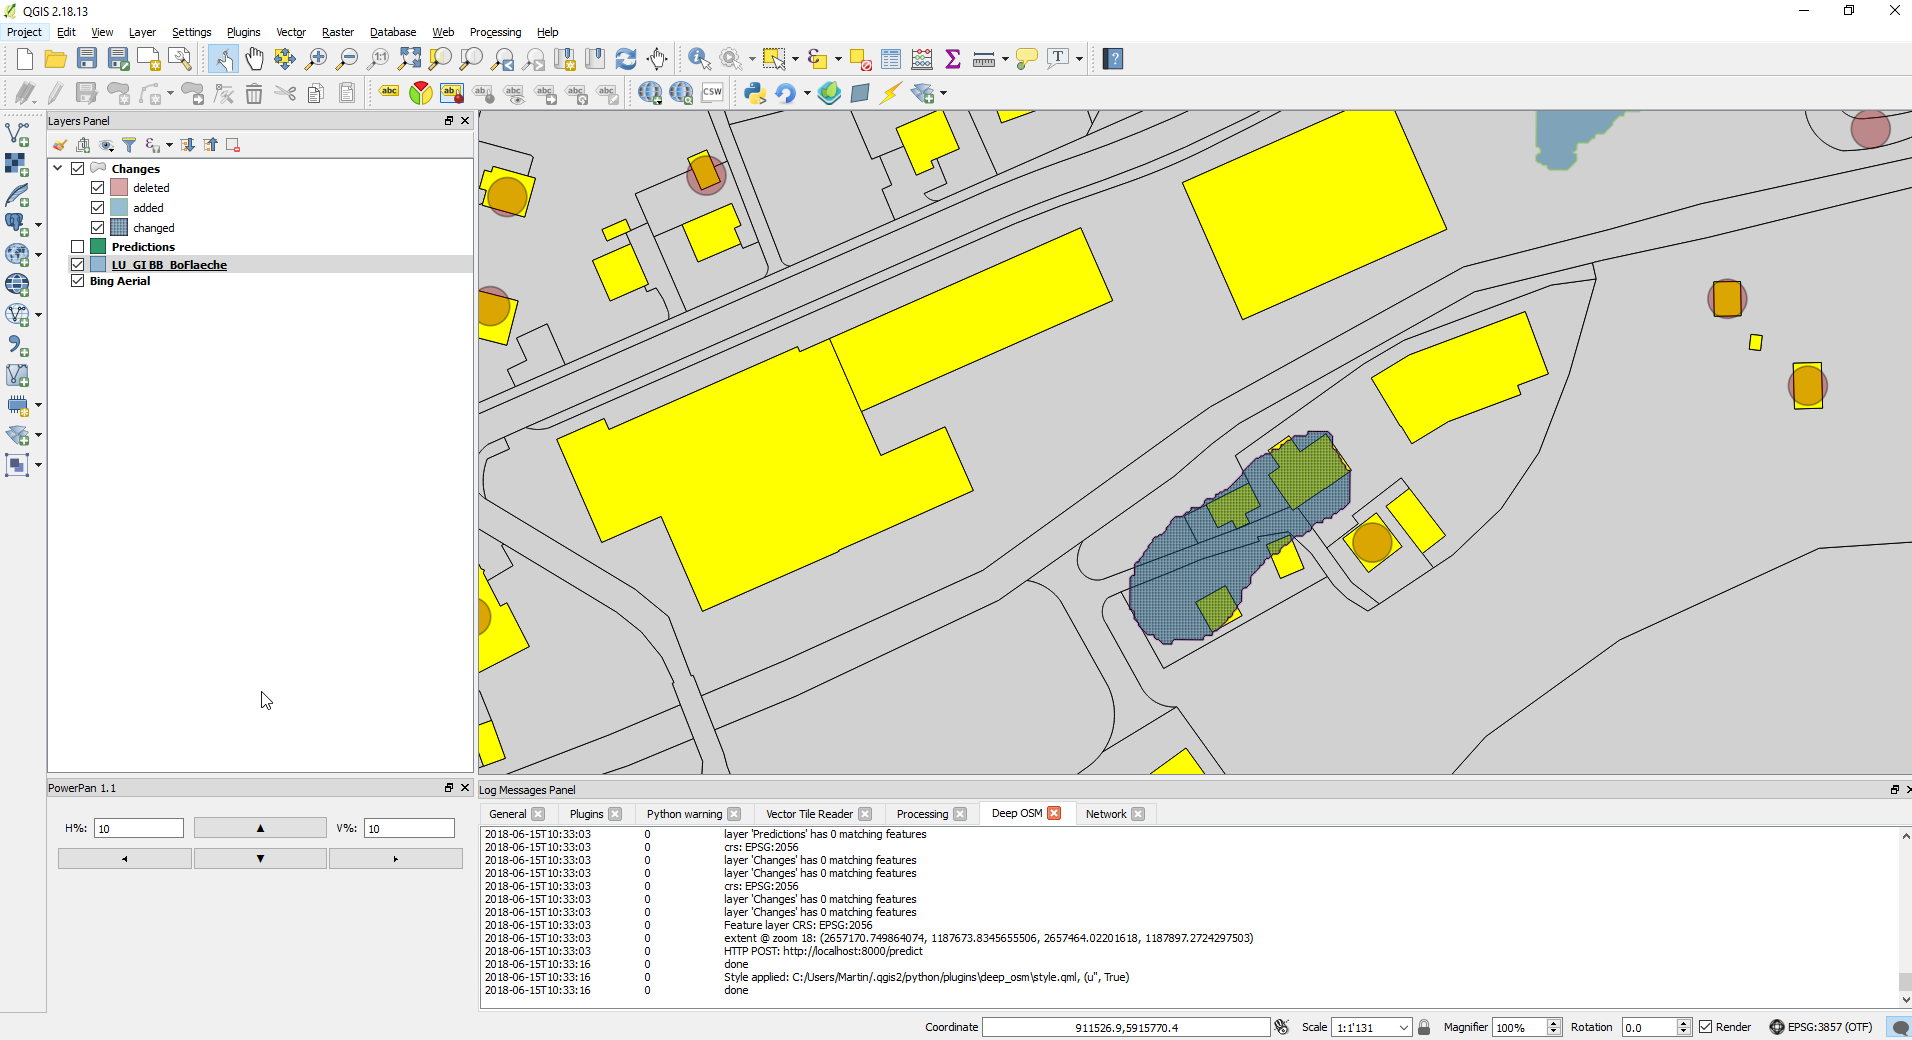
\includegraphics[width=1\linewidth]{chapters/practical_results/images/qgis_changes.png}
	\caption{Changes on cadastral survey data layer}
	\label{fig:plugin:changes_cadastral_layer}
\end{figure}

\begin{figure}[H]
    \centering
	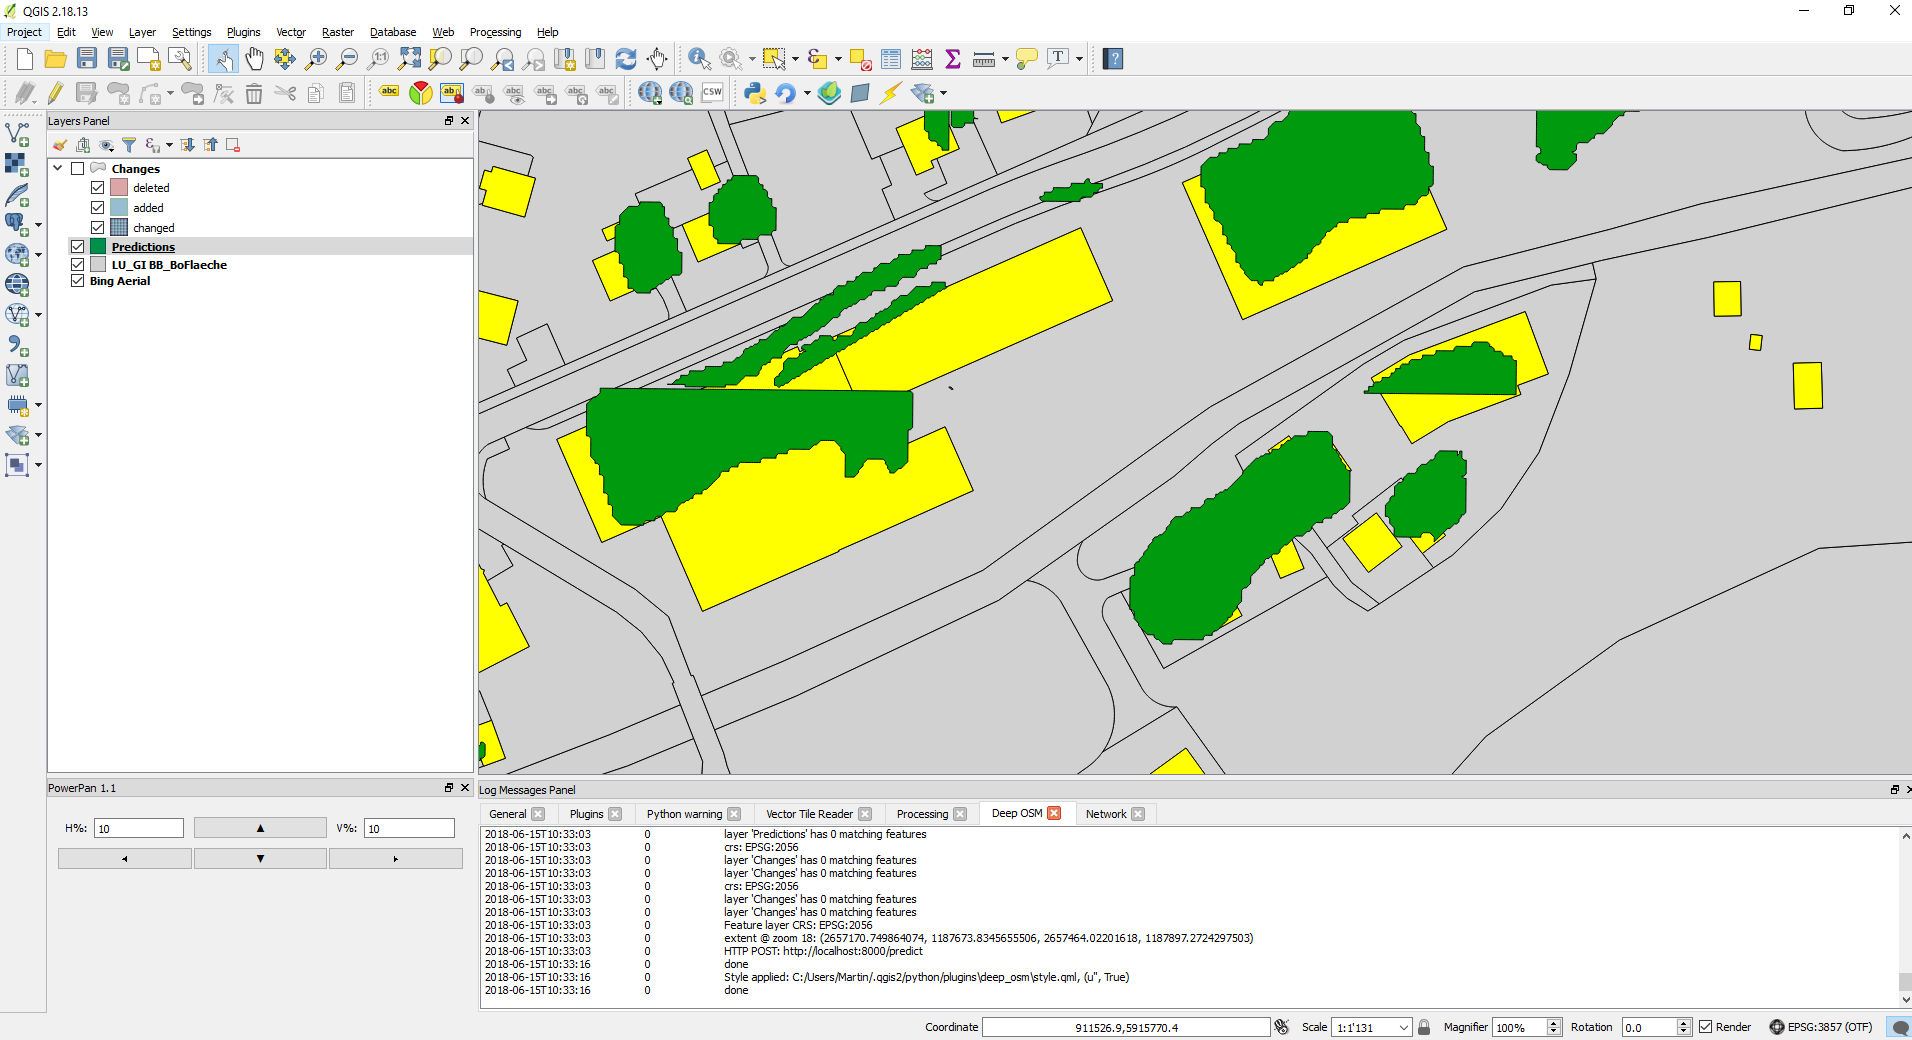
\includegraphics[width=1\linewidth]{chapters/practical_results/images/qgis_predictions.png}
	\caption{Predictions (green) as generated by the neural network}
	\label{fig:plugin:predictions}
\end{figure}

\begin{figure}[H]
    \centering
	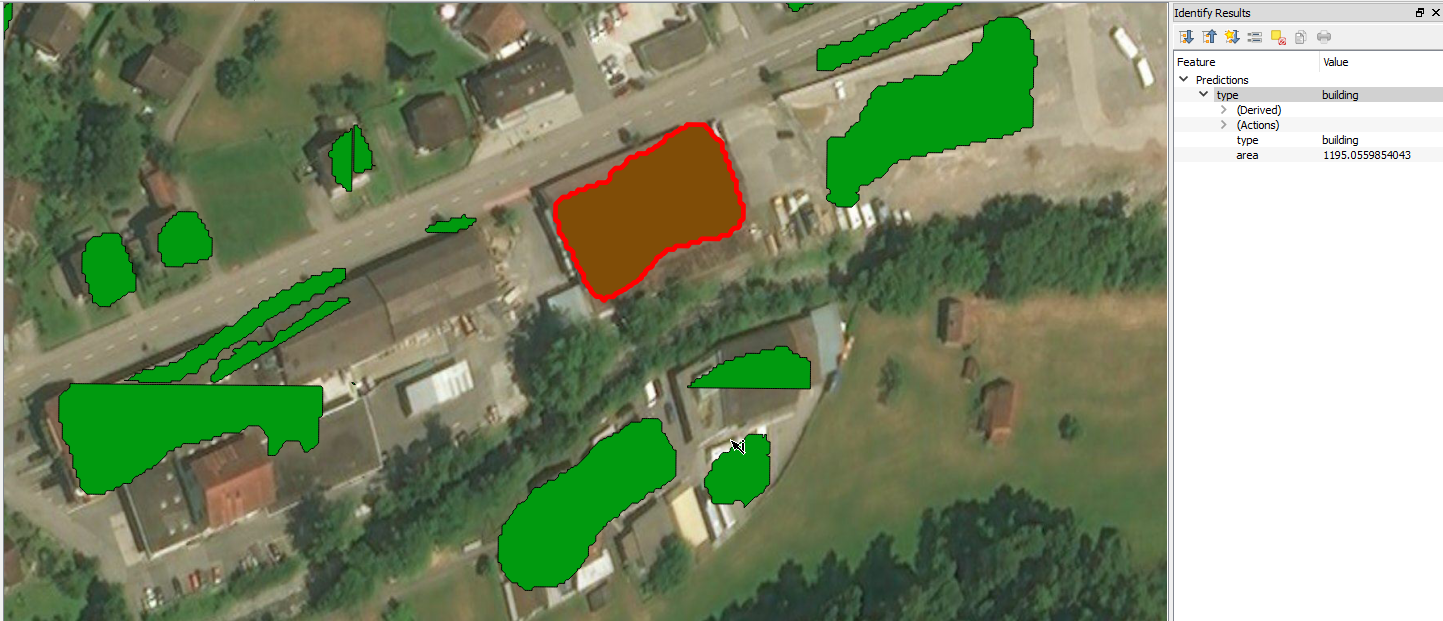
\includegraphics[width=1\linewidth]{chapters/practical_results/images/qgis_prediction_attributes.png}
	\caption{Predictions have attributes showing the predicted class (building in this case)}
	\label{fig:plugin:prediction_attributes}
\end{figure}

\begin{figure}[H]
    \centering
	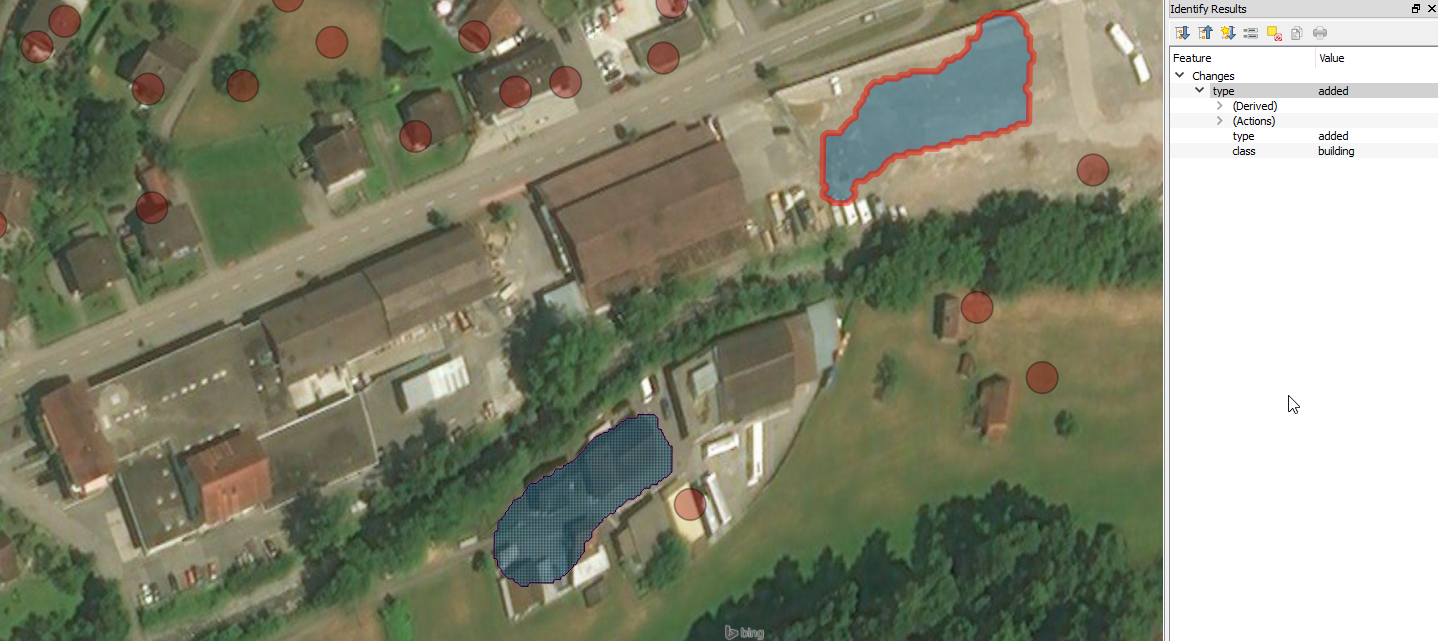
\includegraphics[width=1\linewidth]{chapters/practical_results/images/qgis_changes_attributes.png}
	\caption{Changes have attributes showing the predicted class and the type of change (added, deleted, changed)}
	\label{fig:plugin:change_attributes}
\end{figure}

\section{Prediction Accuracy}
Normally, the accuracy of predictions of objects on orthophotos is measured using \textit{Intersection over Union} (IoU), also called \textit{Jaccard coefficient} \cite{Liu.2011} which is a measure of similarity between objects. Its calculation is shown in \autoref{fig:results:iou}.

\begin{figure}[H]
    \centering
	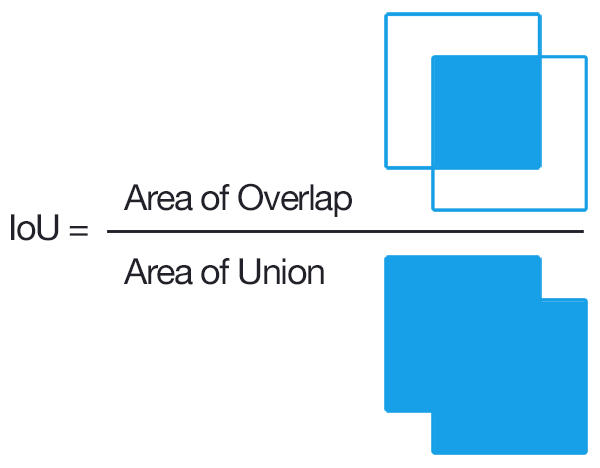
\includegraphics[width=0.6\linewidth]{chapters/practical_results/images/iou_equation.png}
	\caption{The calculation of Intersection over Union (IoU)\\Source: https://www.pyimagesearch.com/2016/11/07/intersection-over-union-iou-for-object-detection/ (23.06.2018)}
	\label{fig:results:iou}
\end{figure}

However, due to its non-differentiability, the IoU can not directly be used as loss-coefficient during the training of the neural network. Despite that, there are options how to use IoU during training shown in \cite{Bebis.2016}, \cite{Yu.20160804}.

Since the goal of this thesis is not to get the most accurate predictions but to reduce the false positives and false negatives as much as possible, it does not really matter if the prediction is extremely accurate but if all objects of their corresponding classes are found. Due to this, we introduce a new metric called \textbf{Hit rate}, which simply counts if an object was found (hit) or not. It can be calculated as shown.

\begin{equation}
	Precision = \dfrac{|TP|}{|TP| + |FP|}
\end{equation}
and
\begin{equation}
	Recall = \dfrac{|TP|}{|TP| + |FN|}
\end{equation}
where:
\begin{itemize}[label=]
    \item $TP$: True positive prediction
    \item $FP$: False positive prediction
    \item $FN$: False negative prediction
\end{itemize}

Finally, accordingly to this metrics, our predictions have a \textbf{Precision of 95.33\%} and a \textbf{Recall of 88.96\%}. This values have been evaluated using a randomly selected batch of 150 images from the test data set.

